\section{Trabajos Relacionados}

El estudio de índices de biomasa ha sido ampliamente registrado por diferentes 
estudios. Muchos de ellos demuestran la utilidad del uso de imágenes
satelitales a diferentes resoluciones. Por lo general, estos estudios parten de un 
trabajo de campo donde se calcula el valor nominal de biomasa a diferentes
muestras haciendo uso de técnicas tradicionales en laboratorio. Posteriormente,
se utilizan estos resultados y las diferentes bandas proveídas por las imágenes
de satélite para inferir un modelo utilizando alguna técnica de regresión que
después es extrapolada al resto del área de estudio.

Por ejemplo, \cite{klemas2013remotesensing} usa esta metodología para detectar cambios en
los niveles de biomasa en diferentes zonas costeras de los Estados Unidos utilizando
imágenes LIDAR y regresión lineal. De forma análoga, \cite{baccini2008afirst}
usa imágenes MODIS y árboles de decisión (en adición a las técnicas
tradicionales de regresión) para estimar el índice AGB (Above-Ground Biomass)
en una extensa área del África tropical. Similiar a este trabajo, \cite{mitchard2009usingsatellite}
utilizan imágenes de radar para predecir AGB en cuatro reservas y parques
nacionales africanos clasificando diferentes tipos de corteza terrestre.
\cite{muukkonen2007biomass} hacen también uso de imágenes MODIS en
conjunto con imágenes ASTER para estimar biomasa con el fin de levantar un
inventario de captura de carbono. Un aporte importante de esta publicación es
que comparten la metodología utilizada durante el proyecto como lo muestra la figura~\ref{fig:Mukkonnen01}. \cite{powell2010quantification}
introducen el uso de nuevas técnicas de regresión (reduced major axis regression,
gradient nearest neighbor imputation y ramdom forest regression trees) para la
generación de modelos de biomasa esta vez analizando imágenes Landsat.
En \cite{hall2006modeling} se introduce bioSTRUCT, un método para generar
correlaciones entre los valores continuos medidos por las bandas de las imágenes
satelitales y el AGB medido previamente usando técnicas de laboratorio. El
artículo ilustra la metodología con un caso de estudio en Alberta (Canada) e
imágenes Landsat ETM+ de libre acceso. Como resultado se obtienen formulas
de regresión a partir de un número limitado de muestras que pueden extrapolarse
al resto del área de estudio.

\begin{figure}
  \centering
  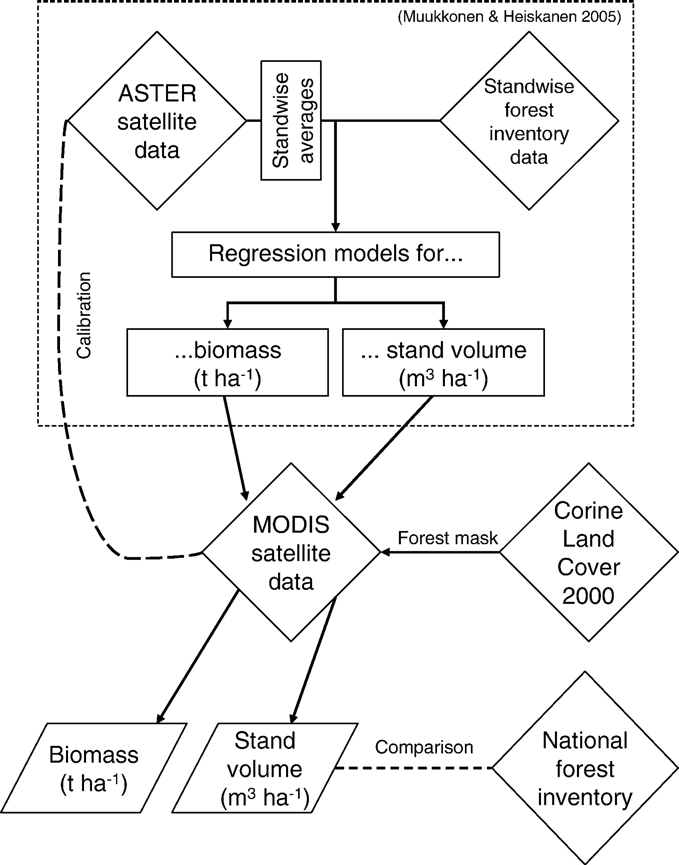
\includegraphics[width = 8cm]{Mukkonnen01.png}
  \caption{Metodología propuesta por \cite{muukkonen2007biomass}}
  \label{fig:Mukkonnen01}
\end{figure}
